\chapter{Literature Review}
\section{Introduction}
In the past decade, conversational chatbots have seen a surge in popularity. Virtual assistants, such as Google Assistant and Amazon Alexa, are now entering our homes via commercial Internet of Things devices. In 2017, Google Assistant was present on over 400 million devices \cite{chandra2018}. Furthermore, specialized chatbots have seen an influx within banking, retail, and healthcare \cite{gvr2017}; chatbots represent a trend towards using natural language in the realm of human-computer interaction (HCI).  This literature review will explore how chatbots are implemented, their benefits, and how this project can implement current technologies to create a novel chatbot application.

\section{Chatbots}
When discussing chatbots, the beginning of their history is usually cited as Alan Turing’s 1950 article “Computing Machinery and Intelligence” \cite{turing1950computing}, wherein Turing describes a test to determine whether a human evaluator can distinguish between a human and a machine during a natural language conversation. This test became known as the Turing test, and poses the question: "Can machines think?". However, the goal of many chatbots is not to create true artificial intelligence, but rather to using pattern matching and conversational responses to mimic the responses of a human.

One of the first programs to attempt the Turing test was ELIZA, created by Joseph Weizenbaum between 1964 and 1966 \cite{weizenbaum1976computer}. ELIZA consisted of a language analyser and a set of rules by which the ‘chatterbot’ followed. ELIZA used a script called DOCTOR was designed to simulate responses of a psychotherapist during a psychiatric interview – predominantly achieved by the therapist mirroring the responses of the patient  \cite{weizenbaum1976computer}. ELIZA may be considered rudimentary and narrow by today’s standards, it forms the basis of our understanding of chatbots and human computer interaction, and how we can teach machines to mimic human characteristics in dialogue.

Another notable development in chatbots and natural language processing is ALICE (Artificial Linguistic Internet Computer Entity), originally implemented in 1995 by Richard Wallace \cite{wallace2009anatomy}. The system won the Loebner Prize three times, a competition inspired by the Turing Test to judge how well a machine can mimic human responses \cite{keedwell2014loebner}. Although the prize itself was met with some criticism -- Shieber critiques that the goal of the Turing Test is lost on the competition \cite{shieber1994lessons} -- ALICE provides a framework for many of the fundamentals we see in modern chatbots and artificial intelligence.

Intelligent virtual assistants (IVA) are conversation agents that allow users to interact with services and Internet of Things (IoT) devices \cite{chung2018intelligent}. IVAs are ubiquitous in modern life, with most smartphones pre-equipped with a virtual assistant such as Google Assistant or Apple Siri. In many ways, IVAs incorporate many functions of chatbots, as well as providing additional features such as voice input and communication with IoT “smart devices”.
\hilight{continue}

Industries are seeing a growing trend in chatbot integration in their business. Autodesk integrated IBM’s Watson Assistant \cite{ibm2017watson} to process 100,000 user support conversations, reducing the resolution time of enquiries from 38 hours to 5.4 minutes \cite{ibm2017autodesk}. Many technology companies offer AI cloud services, many of which allow the integration of chatbots including Watson Assistant and Microsoft Azure Bot Service \cite{microsoft2019azure}. The next section will explore and discuss techniques for implementing chatbots and explore technologies that can be used.

\newpage
\section{Chatbot Models}
A chatbot usually consists of three key components – natural language processing (NLP), response generation (RG) and the knowledge base \cite{cahn2017chatbot}. Generating a response given the context of a conversation is one of the fundamentals of a chatbot system. These models are usually rule-based or learning-based \cite{wang2013dataset}, and each has its advantages and challenges which will be explored in this section.

\subsection{Pattern Matching}
A rule-based model uses pre-defined patterns in order to match an input to a response. This is seen in ALICE, which uses AIML to construct stimulus-response pairs \cite{wallace2009anatomy}. AIML is an XML-based dialect, which defines units of conversation as a category, with a defined input or stimulus known as a pattern. The response is defined within a template \cite{wallace2009anatomy}, and can make use of utilities such as wildcards and states to help the interpreter to perform some logical processing.

Rule-based models are inherently limited by the definitions of its own ruleset, but they can be effective in closed-domain systems where the context of the conversation is known. This method is easier to implement and debug, but may be thrown by unexpected inputs do not match the definitions of the rules. Rule-based models, in particular AIML, are widely-adopted by chatbot platforms such as Pandorabots \cite{pandorabots2019about}.

\subsection{Neural Networks}
When dealing with open-domain conversations, we can use neural networks to train a chatbot model to deal with unexpected inputs and complex multi-step conversations \cite{vinyals2015neural}. Vinyals et al. use the seq2seq framework \cite{sutskever2014sequence}, which is based on recurrent neural networks (RNN), to produce a generative conversational model. The advantage of using an RNN is its reusability for multiple datasets, as well as extract knowledge from noisy datasets, as concluded in \cite{vinyals2015neural}.

\hilight{continue}

The neural network approach has a clear advantage in open-domain conversations, and training from multiple datasets, however the results can be unexpected and can require rigorous debugging.

\newpage
\section{Datasets}
Typically, chatbots are divided into two groups, open-domain and closed-domain \cite{ilievski2018building}. In an open-domain system, the conversation can go in any direction, and the user can talk to the chatbot about any topic. A closed-domain system is restricted to a narrower topic area or set of function – these are the chatbots we see most in real-world applications such as customer service and banking. For this project, the focus will be on a closed-domain system as the goal is to create a chatbot that can achieve a goal – these are often called Goal-Oriented (GO) Chatbots \cite{ilievski2018building}. However, to create a GO chatbot, one must have a goal the chatbot should achieve, and a dataset from which to learn. The selection criteria for this project includes a dataset that is large enough to allow querying and searching, as well as conditionally selecting records that fit the user query. The dataset should also be open to use for research projects, and readily available to access online or download.


\subsection{Ubuntu Dialogue Corpus}
The Ubuntu Dialogue Corpus (UDC) is one of the largest public dialogue datasets available, consisting of 1 million multi-turn dialogues from users receiving technical support for Ubuntu-related problems \cite{lowe2015ubuntu}. This dataset has been used in several dialogue system implementations successfully, as seen in \cite{lowe2015ubuntu} where the dataset is used to compare learning architectures for multi-turn dialogue systems. 

\hilight{Excerpts}

The corpus is widely used in research experiments \cite{kadlec2015improved}, and has been used to train neural network models for more general use \cite{lowe2017training}. However, the drawback of this dataset is its utility and expandability for this project; while it allows us to explore chatbots in a multi-turn context, from an end-user point of view, the average user may not find any use in the information it provides. Furthermore, we are limited to questions around Ubuntu help questions, and it is not ideal for searching and querying the dataset to great effect. 


\subsection{DBPedia}
In terms of knowledge bases which lend themselves to the question and answer format, Wikipedia is the world’s largest collaboratively edited source of encyclopaedic knowledge \cite{volkel2006semantic}. In terms of size, it eclipses the size of the Encyclopaedia Britannica, its nearest rival, by a factor of ten \cite{medelyan2009mining} -- as of 12 November 2019, there are over 5.9 million articles in English, and over 51 million articles in the 306 languages officially covered by the Wikimedia Foundation \cite{wikimedia2019}. However, Wikipedia’s content is only fit for human reading \cite{volkel2006semantic} and is hard to process computationally. Many attempts have been made to formalise and structure this data, as seen in \cite{volkel2006semantic}, \cite{medelyan2009mining}, \cite{wu2007autonomously}, but this review will focus one DBpedia.

DBpedia is a crowd-sourced effort to extract structured content from various Wikimedia projects \cite{dbpedia2019about}, including Wikipedia. The English version of the DBpedia knowledge base describes 4.58 million things, out of which 4.23 million are classified in a consistent ontology, comprising of 320 classes described by 1,650 different properties \cite{dbpedia2019ontology}. This structure enables programs to process this data effectively, including a chatbot application. The size of the DBpedia Ontology is shown in Figure~\ref{fig:ontology}, which demonstrates the scale of the knowledge base, which may be effective for this project.

\begin{figure}[h]
	\begin{center}
		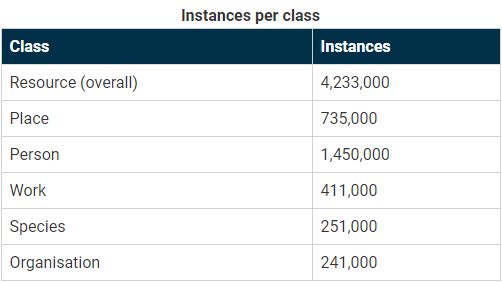
\includegraphics[width=.5\paperwidth]{dbpediaontology}
	\end{center}
	\caption{DBPedia Ontology instances per class \cite{dbpedia2019ontology}}
	\label{fig:ontology}
\end{figure}

The DBpedia extraction framework is responsible for extracting data from Wikipedia into a structured knowledge base, an overview of which is shown in Figure~\ref{fig:extraction}. This extraction is structured into four phases, as described in \cite{lehmann2015dbpedia}:

\begin{itemize}[label={},itemindent=-2em,leftmargin=2em]
	\item {\bf Input:} Wikipedia pages are read from an external source, either from a Wikipedia dump, or using the MediaWiki API.
	\item {\bf Parsing:} Each Wikipedia page is parsed, which transforms the source code of the Wikipedia page into an Abstract Syntax Tree (AST). An AST is a tree representation of the syntactic structure of the source code.
	\item {\bf Extraction:} The Abstract Syntax Tree of each page is forwarded to the extractors. There are many types of extractors, which will later be described, which extract data such as labels, images and infoboxes. Each extractor takes an AST as input and yields a set of Resource Description Framework (RDF) statements. These are XML statements which describe properties and values of resources.
	\item {\bf Output:} These RDF statements are written into sinks, which receive the data.
\end{itemize}

\begin{figure}[h]
	\begin{center}
		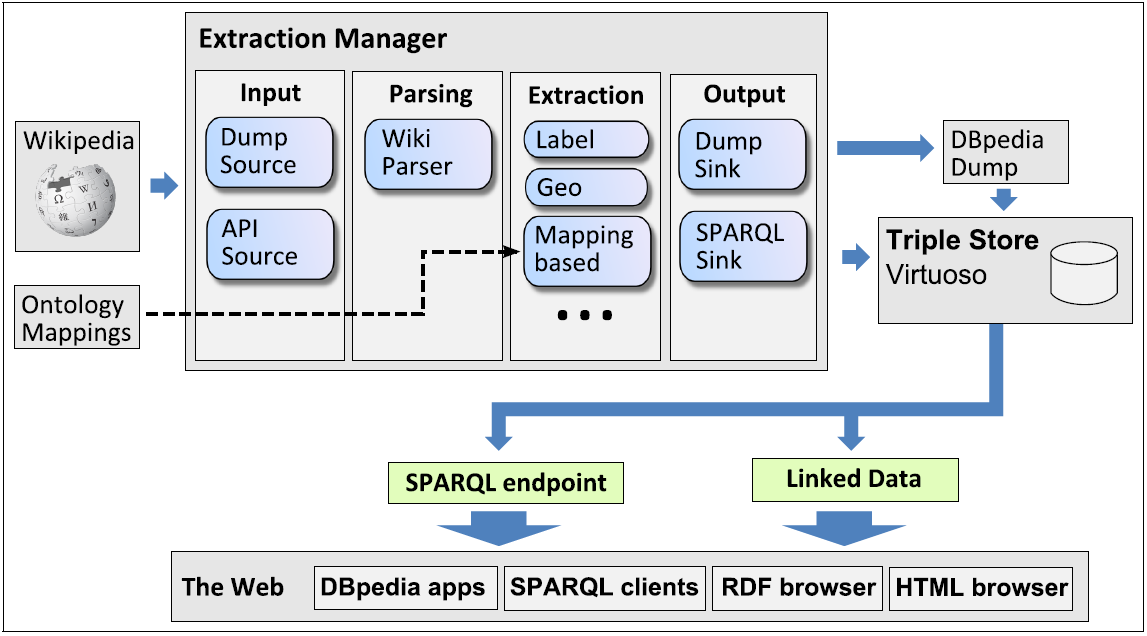
\includegraphics[width=.6\paperwidth]{dbpediaextraction}
	\end{center}
	\caption{DBpedia extraction framework \cite{bizer2009dbpedia}}
	\label{fig:extraction}
\end{figure}

The DBPedia ontology organises its entities using RDF models, each of which has many properties and are linked to subclasses and super-classes where necessary. This can be seen in Table~\ref{tab:ontology}, where a subclass may inherit the properties of its parent class. This can assist querying and searching, as we can query based on properties of a given class, as well as filtering and matching with conditional queries. 
\newpage
\begin{table}[h]
	\centering
	\begin{tabular}{{@{}lll@{}}}
		\toprule
		Ontology class & Instances & Example properties \\
		\midrule
		Person & 198,056 & name, birthdate, birthplace, employer, spouse \\
		\hspace{3mm} Artist & 54,262 & activeyears, awards, occupation, genre \\
		\hspace{6mm} Actor & 26,009 & academyaward, goldenglobeaward, activeyears \\
		\hspace{6mm} MusicalArtist & 19,535 & genre, instrument, label, voiceType, activeyears \\

		Athlete & 74,832 & currentTeam, currentPosition, currentNumber \\

		Politician & 12,874 & predecessor, successor, party \\
		\bottomrule
	\end{tabular}
	\caption{Example DBPedia classes and example instances \cite{lehmann2015dbpedia}}
	\label{tab:ontology}
\end{table}

The data extracted is mapped to the ontology classes and properties to provide structured RDF statements. This allows instances of classes to be queried using SPARQL ...\\ 
\hilight{continue: Semantic Web, code example, endpoints}

\subsection{Other Candidates}

\newpage
\section{Programming Languages}
At its core, the language used to implement a chatbot has few criteria; it needs to be able to process natural language, provide a user interface for input and output, and can optionally interact with a data source. A bare minimum chatbot could therefore be implemented with virtually any programming language. However, it is important to consider the capabilities of the language, including support for machine learning, database interactions and user interface designs. This section will compare programming technologies based on their performance, their compatibility with the chatbot models previously discussed in the report, and the availability of libraries and functionality which may be useful for implementing a fully-featured, extensible chatbot.
 
\subsection{Python}
Python has been widely adopted in the scientific industry [31], touted for its extensive collection of scientific libraries [32]; it recently eclipsed Java to become the most popular language, according to IEEE Spectrum [33]. Natural language processing can be quickly implemented with libraries such as Natural Language Toolkit (NLTK) [34]; artificial neural networks (ANNs) can be leveraged with many libraries, including Scikit-learn [35]. Newer developments in machine learning include TensorFlow [36], which provides a novel learning framework utilised for large scale ML implementations such as healthcare [37] and Google’s own search engine [38]. In the chatbot realm, Python allows for interpretation of AIML with the python-aiml library [39]; more comprehensive chatbot libraries can also be utilised, such as ChatterBot [40]. Using Python would therefore provide the freedom to explore various technologies for implementing the project and extend the functionality in the future, given the abundance of relevant libraries.

In the context of linking data sources, the database access layer in Python is inherently weaker than other technologies such as JDBC and ODBC [41]. However, this is mainly a concern for enterprise solutions, as Python’s DB-API specification can connect to most databases [42]. Furthermore, connecting to a SPARQL endpoint and parsing RDF graphs is possible through RDFLib [43]. Many Python web frameworks can handle user interaction, routing, and security. Some of the popular web frameworks include Django, TurboGears, and Flask [44]. These frameworks vary in their features and quirks, but for the scale of this project, it is safe to assume that any of them will fit the criteria and they can be explored further in the experimentation phase.
Python has been used extensively in the machine learning field, and can be seen in many Machine Learning as a Service (MLaas) services; the Microsoft Azure Machine Learning service uses Python for training and modelling [45]. \hilight{continue}

\subsection{Java}
Java is widely used in machine learning implementations [46] [47], and is prevalent in research and enterprise solutions. Many libraries exist to implement machine learning frameworks [48], natural language processing [49], and AIML interpreters [50]. Java has the advantage of being truly cross-platform since the Java program is compiled into byte-code to be interpreted by the Java virtual machine [46]; this may beneficial to this project if it is deployed to a Linux web server, for example.\\
\hilight{RDF/Jena, Web, Performance}

\subsection{Clojure}
Lisp - Pandorabots

\subsection{Analysis}

\cleardoublepage
\section{Existing Solutions}
Dialogue systems are abundant in business and consumer use, from ordering pizza with your Google Home device [51] to diagnosing and managing patients’ medical conditions [52]. This section will explore existing solutions that are relevant to the scope of this project, as well as broader chatbot platforms currently in use.

\subsection{Google Assistant}
\subsection{DBPedia Chatbot}
\subsection{Mitsuku}
\label{subsec:Mitsuku}

\subsection{DBPedia Spotlight}

\section{Related Work}

\section{Conclusion}





